\documentclass[12pt]{ltjsarticle}

\usepackage[T1]{fontenc}
\usepackage[utf8]{inputenc}
\usepackage[backend=biber, maxnames=100, backref=true]{biblatex}
\usepackage[binary-units = true]{siunitx}
\usepackage{amsmath, amssymb, amsthm}
\usepackage{graphicx}
\usepackage{hyperref}
\usepackage{ascmac}

\DeclareGraphicsRule{.ai}{pdf}{.ai}{}

\newcommand*{\exref}[1]{例~\ref{#1}}
\newcommand*{\fgref}[1]{図~\ref{#1}}

\newtheorem{example}{例}
\newtheorem{theorem}{定理}
\newtheorem{lemma}{補題}

\addbibresource{reference.bib}

\begin{document}
\section{瞬時復号可能な符号}
瞬時復号可能な符号とは, 名前の通り, 符号がやってきたらそれを瞬時に復号可能な符号のことをいう.
これはつまり, 全てのメッセージを受信してから復号を行うのではなく, 来た時点で遅延なく復号可能な符号のことをいうのである.
厳密に言えば, 符号$\mathcal{C}$が\textbf{瞬時復号可能な符号}(instantaneously decodable code)あるいは\textbf{瞬時符号}(instantaneous code)であるとは,
各符号列$w_{i_1}, w_{i_2}, \cdots, w_{i_n}$に対し,
$\boldsymbol{t} = w_{i_1} w_{i_2} \cdots w_{i_n} \cdots$で始まる全ての符号列が
$\boldsymbol{s} = s_{i_1} s_{i_2} \cdots s_{i_n} \cdots$として一意に復号され,
その後に続く$\boldsymbol{t}$のシンボル列に無関係なことをいう.
\begin{example} \label{ex:not-uniquely}
  2元符号$\mathcal{C}$
  \begin{align*}
    s_1 \mapsto 0, s_2 \mapsto 10, s_3 \mapsto 11
  \end{align*}
  は瞬時復号可能な符号, つまり, メッセージ$\boldsymbol{t}$を受信しながら復号できる.
  なぜならば, $0$が来れば$s_1$に復号可能であるし, $1$が来れば, 次に来る符号を見てすぐに$s_2$なのか$s_3$なのかを判定できる.
\end{example}
\begin{example}
  2元符号$\mathcal{C}$
  \begin{align*}
    s_1 \mapsto 0, s_2 \mapsto 01, s_3 \mapsto 11
  \end{align*}
  は瞬時復号可能ではない.
  たとえば, $\boldsymbol{t} = 01111 \cdots$というメッセージが来たとき,
  $\boldsymbol{t} = 0.11.11.11. \cdots$なのか$\boldsymbol{t} = 01.11.11.11. \cdots$なのかはすぐには判定できず, メッセージ長が奇数か偶数かを見なければ判定することはできない.
\end{example}

一般に, 瞬時符号であれば一意復号可能な符号であることは成立するが, 逆は成立しない.
例えば, \exref{ex:not-uniquely}で定義する符号は一意復号可能だが, 既に見たように瞬時復号可能ではない.

符号$\mathcal{C}$が\textbf{語頭符号}(prefix code)であるとは, どの符号語$w_i$も他の符号$w_j \enspace (i \neq j)$の語頭にないことをいう.
すなわち
\begin{align*}
  \forall w \in T^*, w_j \neq w_i w
\end{align*}
である.
また, $C_1 = \emptyset$とも言い換えることもできる.
この語頭符号と瞬時符号との間には次のような関係がある.
\begin{screen}
  \begin{theorem}
    符号$\mathcal{C}$が瞬時符号であることと, 語頭符号であることは同値.
  \end{theorem}
\end{screen}
\begin{proof}
  まず, $\mathcal{C}$が瞬時符号であるとして, 語頭符号となることを示す.
  $\mathcal{C}$が語頭符号でないとする.
  このとき, ある$w_j$の語頭に$w_i$という符号列が含まれる.
  すると, $\boldsymbol{t} = w_i \cdots$で始まる符号列は$\boldsymbol{s} = s_i \cdots$にも,
  $\boldsymbol{s} = s_j \cdots$にも復号化される.
  よって, 符号$\mathcal{C}$は瞬時符号ではないが, $\mathcal{C}$が瞬時符号であることに矛盾.
  以上から, 符号$\mathcal{C}$は瞬時符号であれば, 語頭符号となる.

  次に, $\mathcal{C}$が語頭符号であれば, 瞬時符号でもあることを確認する.
  $\mathcal{C}$が語頭符号なので, $\boldsymbol{t} = w_i \cdots$であれば,
  この符号列は$\boldsymbol{s} = s_i \cdots$に復号化されなければならない.
  これは$w_i$は他の$w_j \enspace (i \neq j)$の語頭とはならないために, 一意に復号化されるためである.
  よって, どの符号列に対してもこの事実が成立するので,
  全てのシンボル列は$\boldsymbol{t}$の後続のシンボル列とは無関係となる.
  以上から, $\mathcal{C}$は瞬時符号となる.
\end{proof}

\section{瞬時符号の構成法}
$r$元瞬時符号は$r$分木によって構成することができる.
ここで考える$r$分木は\fgref{eq:r-ary-tree}のようにより根に空語$\epsilon$を配置し,
それに各シンボルを1つだけ加えたものを根の子にそれぞれ追加し,
以下同様にシンボルを1つずつ加えたものをそれぞれ子に...ということを繰り返す.
\begin{example}
  \label{ex:make-tree}
  語長を$4$までとしたときに構成される2分木は\fgref{fg:binary-tree}の通り.
  \begin{figure}
    \centering
    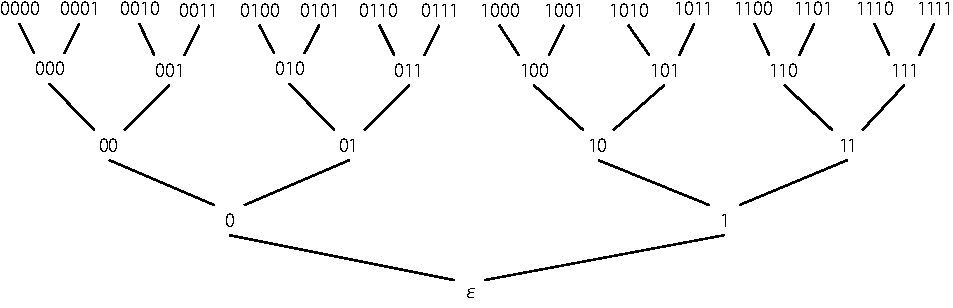
\includegraphics{image/2分木.pdf}
    \caption{語長$4$のときの2分木. 必ず根に近いノードの方をそのノード以降のノードは語頭として持っている.}
    \label{fg:binary-tree}
  \end{figure}
\end{example}

このようにして作った$r$分木に対して, 先程の語頭符号と瞬時符号が同値である命題を使い,
望む瞬時符号を構成していく.
まず, $r$分木のノードを1つ選ぶ.
次に, 選んだノード以降のノードを刈り込む(選んだノードの子や孫を削除する).
すなわち, 選んだノードを語頭に含んでいるノードを全て木から削除する.
これを繰り返すことで, 最終的に瞬時符号を構成することができる.
\begin{example}
  \exref{ex:make-tree}の中から$0, 10, 110, 1110, 1111$を符号語とした符号は瞬時符号となる.
  \fgref{fg:processed-binary-tree}の通り,
  選択したノードが必ず他の語を語頭とならないよう刈り込みがなされている.
  \begin{figure}
    \centering
    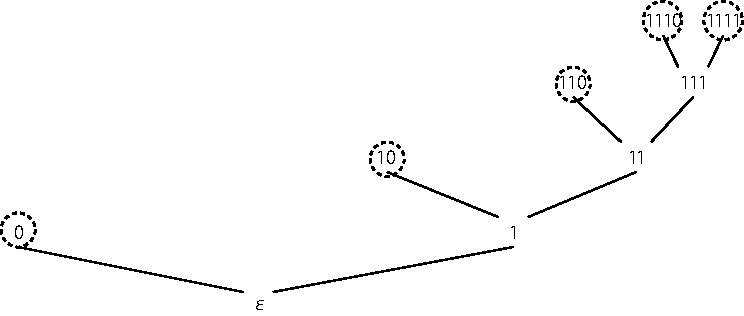
\includegraphics{image/構成された瞬時符号.pdf}
    \caption{\exref{ex:make-tree}からいくつか刈り込んで瞬時符号を構成している例. 符号として選ばれたノードは円で囲まれている.}
    \label{fg:processed-binary-tree}
  \end{figure}
\end{example}

\section{クラフトの不等式}

\printbibliography[title=参考文献]
\end{document}
